% !TeX root = ../tg.tex
\chapter{实验部分}
\section{分割-联邦学习收敛性的实验验证}
\subsection{实验设置}
我们在 CIFAR-10 和 CIFAR-100数据集上进行了实验。 两个数据集均包含 6 万张图像（5 万张用于训练，1 万张用于测试），不同之处在于 CIFAR-10 包含 10 个类别，而 CIFAR-100 包含 100 个类别。我们使用交叉熵作为损失函数。

为了模拟数据异构性，我们采用了广泛使用的 Dirichlet 分布 \cite{hsu2019measuring}，并引入一个控制参数 $\alpha$。其中，较小的 $\alpha$ 值表示客户端之间的数据异构性更高。我们选用 ResNet-18 作为模型结构，该网络包含四个残差块，并考虑四种模型切分方式，分别由 $L_c=\{1,2,3,4\}$ 表示，其中 $L_c=n$ 表示模型在第 $n$ 个残差块之后进行切分。

我们将两种主流分布式学习方法作为基准进行比较：联邦学习（FL，特别是 FedAvg \cite{mcmahan2017communication}）和分割学习（SL）\cite{vepakomma2018split}。SFL-V1、SFL-V2、FL 和 SL 的学习率统一设置为 $0.01$。批量大小 $b_s = 128$，实验运行总轮数为 $T=200$ 轮。

我们使用以下参数设置：客户端数量 $N=10$，数据异构性参数 $\beta=0.1$，本地训练轮数 $E=5$，其中 $E$ 表示客户端模型聚合前的本地训练次数（即每对每个客户端的数据进行 $E$ 次训练后，其客户端侧模型将在联邦服务器上进行聚合），因此 $\tau=\lceil \frac{D_n}{b_s}\rceil\times E$。为了与标准联邦学习进行公平比较，我们将 $\tau$ 设置为与 $\tilde{\tau}$ 相等。
所有实验运行在 CPU（Intel(R) Xeon(R) Gold 5320 @ 2.20GHz）和 GPU（A100-PCIE-80GB）平台上。
\subsection{实验结果}
在分割-联邦学习中，各类超参数豆会对于模型的收敛产生影响，本部分实验目标是验证分割-联邦学习在不同超参数下的收敛规律。

每轮训练时数据的迭代次数$E$是可以选择的。一般而言，$E$的值过小可能导致用户的模型在没有学习到足够的信息时就
被联邦服务器聚合，学到的信息也随之消散；$E$的值过大可能导致用户的模型在非独立同分布的数据上产生过大的偏差，联邦服务器无法
将大量存在过大偏差的模型聚合为无偏差的模型。本文选择$E \in \{2,5,10\}$三个值进行实验。根据图\ref{fig:multi-image9}显示，模型的最终准确率
相差无几，但$E=2$时模型的收敛速率更快。
\begin{figure}[H]
\centering
\subcaptionbox{SFL-V1\label{fig:subfi}}
{
\includegraphics[width=0.4\linewidth]{E.pdf}}
\subcaptionbox{SFL-V2\label{fig:sub}}
{
\includegraphics[width=0.4\linewidth]{E (1).pdf}}
\caption{每轮训练数据迭代次数E对准确率的影响}
\label{fig:multi-image9}
\end{figure}

参与训练的用户数$N$也会对模型的准确率产生很大的影响。用户数量较少时，每一个用户可以在
全局模型中占有较大的比重，可以提升全局模型在所有用户上的泛化能力。但同时全局模型也可能被不均匀的数据严重
影响，导致准确率低下。用户数量较多时，每一个用户的模型在全局模型中的比重降低，会降低全局模型的泛化能力。但同时，
单个用户的不均匀数据对全局模型的影响也会降低。本文选择$N\in\{10,50,100\}$三个值进行实验。根据图\ref{fig:multi-image00}显示模型的最终准确率差别不大，
$N$越大时模型的收敛速率越慢。
\begin{figure}[H]
\centering
\subcaptionbox{SFL-V1\label{fig:subfin}}
{
\includegraphics[width=0.4\linewidth]{N.pdf}}
\subcaptionbox{SFL-V2\label{fig:subn}}
{
\includegraphics[width=0.4\linewidth]{N (1).pdf}}
\caption{参与训练的用户数$N$对准确率的影响}
\label{fig:multi-image00}
\end{figure}
每轮参与训练的用户比例$q$会显著影响模型的准确率和收敛速率。当每轮参与训练的比例过低时，
模型每轮难以学习到足够的信息，且模型获得的信息总是带有偏向性的，这种情况会严重影响模型的训练。本文选择$q\in\{0.2,0.5,1\}$
三个值进行实验。根据图\ref{fig:multi-image0000}显示，随着q的增大，模型的收敛速率加快的同时，最终准确率也会提高。
\begin{figure}[H]
\centering
\subcaptionbox{SFL-V1\label{fig:subfiq}}
{
\includegraphics[width=0.4\linewidth]{q.pdf}}
\subcaptionbox{SFL-V2\label{fig:subq}}
{
\includegraphics[width=0.4\linewidth]{q (1).pdf}}
\caption{每轮参与训练的用户比例$q$对准确率的影响}
\label{fig:multi-image0000}
\end{figure}

\section{分割-联邦学习鲁棒性算法的实验验证}

\subsection{实验设置}
客户端数据同样采用Dirichlet分布进行采样，并且也引入控制参数 $\alpha$\cite{hsu2019measuring}。其中，$\alpha$ 的值越大，表示数据异构性越低。我们考虑两种场景：独立同分布（IID，$\alpha=\infty$）和非独立同分布（non-IID，$\alpha=0.1$）。与 \cite{b9,ji2024fedfixer,li2024feddiv} 类似，我们通过随机翻转标签的方式模拟标签噪声，即以一定概率（称为噪声率）将样本的标签随机翻转为其他类别。我们在 CIFAR-10 和 CIFAR-100 数据集上设置了 $\{0, 10\%, 20\%, 30\%, 40\%, 50\%, 60\%\}$ 的噪声率，在 Fashion-MNIST 上设置了 $\{40\%, 50\%, 60\%, 70\%, 80\%\}$ 的噪声率。为了便于观察实验结果，我们仅展示了部分噪声设置下的实验结果。

用于训练 SFL 模型的数据集、模型结构以及客户端数量如表 \ref{table:hyper-parameters} 所示。
主要的超参数如下：批量大小设为 128；学习率为 $\eta^r=0.01$；每轮训练使用 $E=5$ 个 epoch。
我们使用交叉熵作为损失函数。实验所用 GPU 为 A100-80GB，每次训练仅使用一块 GPU。
\begin{table}[t]
\caption{不同数据集的设置}
\begin{center}
\begin{tabular}{cccc}
\hline
数据集 & CIFAR-10 & CIFAR-100 & Fashion-MNIST \\ \hline
客户端数量 & 100 & 100 & 50 \\ 
模型 & ResNet-18 & ResNet-34 & 10层CNN \\ \hline
\end{tabular}
\label{table:hyper-parameters}
\end{center}
\end{table}
\subsection{SFL-DCT的结果}

我们现在评估所提出算法 SFL-DCT 的性能。我们假设在此场景下有 60\% 的客户端存在标签噪声\cite{b9,ji2024fedfixer,li2024feddiv}。我们将 SFL-DCT 与两种现有的去噪算法（FedCorr\cite{b9} 和 FedNoRo\cite{wu2023fednoro}）以及两种基线算法（SFL-V2 和 SFL-V1/FL）\footnote{由于 SFL-V1 与 FedAvg 在逻辑上是相同的算法，因此 SFL-V1 的结果也可以代表 FedAvg。}\cite{thapa2022splitfed} 进行了比较。为了公平比较，我们将这些现有去噪算法转换为基于分割-联邦学习的形式。具体来说，模型被划分为客户端和服务器两部分，训练过程遵循图~\ref{fig:sfl} 中所示的步骤 1 - 步骤 4。在模型聚合阶段，仅对客户端侧模型进行联邦更新，如图~\ref{fig:sfl} 中步骤 5 所示。


表 \ref{table:compare cifar10}、\ref{table:compare cifar100} 和 \ref{table:compare fmnist} 分别展示了不同算法在 CIFAR-10、CIFAR-100 和 Fashion-MNIST 数据集上的平均最佳准确率（3 次实验取平均）。我们观察到，不论用户间的数据是否独立同分布，标签噪声对 SFL-DCT 的影响均小于基线算法（即 SFL-V2 和 SFL-V1/FL）。这是因为 SFL-DCT 能够有效检测并纠正标签，从而显著减轻由标签噪声带来的性能下降。与这两种去噪算法（FedCorr 和 FedNoRo）相比，SFL-DCT 在各种设置下均展现出更优的性能。在数据独立同分布场景下，大多数情况下 SFL-DCT 的准确率略高于这两个竞争算法；而在数据非独立同分布场景下，其表现明显优于它们，体现出更强的鲁棒性和更高的准确性。
\begin{table*}[t]
\caption{CIFAR-10 数据集上各算法的最佳平均准确率}
\begin{center}
\resizebox{\textwidth}{!}{
\begin{tabular}{c|cccccccccccc}
\hline\hline
\multicolumn{1}{c|}{\multirow{3}{*}{算法}} & \multicolumn{12}{c}{测试准确率(\%)} \\ \cline{2-13} 
\multicolumn{1}{c|}{} & \multicolumn{6}{c|}{IID} & \multicolumn{6}{c}{Non-IID} \\ \cline{2-13} 
\multicolumn{1}{c|}{} & \multicolumn{1}{c|}{$\delta$ = 0.1} & \multicolumn{1}{c|}{$\delta$ = 0.2} & \multicolumn{1}{c|}{$\delta$ = 0.3} & \multicolumn{1}{c|}{$\delta$ = 0.4} & \multicolumn{1}{c|}{$\delta$ = 0.5} & \multicolumn{1}{c|}{$\delta$ = 0.6} & \multicolumn{1}{c|}{$\delta$ = 0.1} & \multicolumn{1}{c|}{$\delta$ = 0.2} & \multicolumn{1}{c|}{$\delta$ = 0.3} & \multicolumn{1}{c|}{$\delta$ = 0.4} & \multicolumn{1}{c|}{$\delta$ = 0.5} & \multicolumn{1}{c}{$\delta$ = 0.6} \\ \hline
SFL-DCT & \multicolumn{1}{c}{84.66} & \multicolumn{1}{c}{\textbf{83.84}} & \multicolumn{1}{c}{\textbf{83.15}} & \multicolumn{1}{c}{\textbf{83.15}} & \multicolumn{1}{c}{\textbf{83.07}} & \multicolumn{1}{c}{\textbf{82.07}} & \multicolumn{1}{c}{\textbf{67.20}} & \multicolumn{1}{c}{\textbf{68.31}} & \multicolumn{1}{c}{\textbf{66.15}} & \multicolumn{1}{c}{\textbf{63.12}} & \multicolumn{1}{c}{\textbf{63.33}} & \multicolumn{1}{c}{\textbf{60.99}} \\ 
SFL-V1 & \multicolumn{1}{c}{84.26} & \multicolumn{1}{c}{78.29} & \multicolumn{1}{c}{75.50} & \multicolumn{1}{c}{70.84} & \multicolumn{1}{c}{66.01} & \multicolumn{1}{c}{63.35} & \multicolumn{1}{c}{62.18} & \multicolumn{1}{c}{56.30} & \multicolumn{1}{c}{50.97} & \multicolumn{1}{c}{45.13} & \multicolumn{1}{c}{41.62} & \multicolumn{1}{c}{38.75} \\ 
SFL-V2 & \multicolumn{1}{c}{84.33} & \multicolumn{1}{c}{78.90} & \multicolumn{1}{c}{74.99} & \multicolumn{1}{c}{70.92} & \multicolumn{1}{c}{67.57} & \multicolumn{1}{c}{64.83} & \multicolumn{1}{c}{65.72} & \multicolumn{1}{c}{59.13} & \multicolumn{1}{c}{53.31} & \multicolumn{1}{c}{47.43} & \multicolumn{1}{c}{43.78} & \multicolumn{1}{c}{40.98} \\ 
FedCorr & \multicolumn{1}{c}{\textbf{84.95}} & \multicolumn{1}{c}{83.11} & \multicolumn{1}{c}{82.90} & \multicolumn{1}{c}{82.63} & \multicolumn{1}{c}{82.11} & \multicolumn{1}{c}{81.46} & \multicolumn{1}{c}{63.71} & \multicolumn{1}{c}{57.36} & \multicolumn{1}{c}{51.10} & \multicolumn{1}{c}{46.92} & \multicolumn{1}{c}{41.60} & \multicolumn{1}{c}{39.68} \\ 
FedNoRo & \multicolumn{1}{c}{84.37} & \multicolumn{1}{c}{81.71} & \multicolumn{1}{c}{81.02} & \multicolumn{1}{c}{79.35} & \multicolumn{1}{c}{77.58} & \multicolumn{1}{c}{76.14} & \multicolumn{1}{c}{58.43} & \multicolumn{1}{c}{54.19} & \multicolumn{1}{c}{52.74} & \multicolumn{1}{c}{48.90} & \multicolumn{1}{c}{44.54} & \multicolumn{1}{c}{40.76} \\ \hline
\end{tabular}
}
\label{table:compare cifar10}
\end{center}
\end{table*}
\begin{table*}[t]
\caption{Fashion-MNIST 数据集上各算法的测试准确率}
\begin{center}
\resizebox{\textwidth}{!}{
\begin{tabular}{l|llllllllll}
\hline\hline
\multicolumn{1}{c|}{\multirow{3}{*}{算法}} & \multicolumn{10}{c}{测试准确率(\%)} \\ \cline{2-11} 
\multicolumn{1}{c|}{} & \multicolumn{5}{c|}{IID} & \multicolumn{5}{c}{Non-IID} \\ \cline{2-11} 
\multicolumn{1}{c|}{} & \multicolumn{1}{c|}{$\delta$ = 0.4} & \multicolumn{1}{c|}{$\delta$ = 0.5} & \multicolumn{1}{c|}{$\delta$ = 0.6} & \multicolumn{1}{c|}{$\delta$ = 0.7} & \multicolumn{1}{c|}{$\delta$ = 0.8} & \multicolumn{1}{c|}{$\delta$ = 0.4} & \multicolumn{1}{c|}{$\delta$ = 0.5} & \multicolumn{1}{c|}{$\delta$ = 0.6} & \multicolumn{1}{c|}{$\delta$ = 0.7} & \multicolumn{1}{c}{$\delta$ = 0.8} \\ \hline
SFL-DCT & \multicolumn{1}{c}{\textbf{89.31}} & \multicolumn{1}{c}{\textbf{89.42}} & \multicolumn{1}{c}{\textbf{88.95}} & \multicolumn{1}{c}{\textbf{88.81}} & \multicolumn{1}{c}{\textbf{87.94}} & \multicolumn{1}{c}{\textbf{84.47}} & \multicolumn{1}{c}{\textbf{83.68}} & \multicolumn{1}{c}{\textbf{84.67}} & \multicolumn{1}{c}{\textbf{79.80}} & \multicolumn{1}{c}{\textbf{80.22}} \\ 
SFL-V1 & \multicolumn{1}{c}{85.12} & \multicolumn{1}{c}{84.63} & \multicolumn{1}{c}{84.55} & \multicolumn{1}{c}{83.71} & \multicolumn{1}{c}{83.68} & \multicolumn{1}{c}{74.82} & \multicolumn{1}{c}{71.61} & \multicolumn{1}{c}{66.43} & \multicolumn{1}{c}{64.26} & \multicolumn{1}{c}{64.07} \\ 
SFL-V2 & \multicolumn{1}{c}{86.07} & \multicolumn{1}{c}{85.78} & \multicolumn{1}{c}{85.14} & \multicolumn{1}{c}{84.05} & \multicolumn{1}{c}{83.84} & \multicolumn{1}{c}{75.78} & \multicolumn{1}{c}{72.68} & \multicolumn{1}{c}{66.86} & \multicolumn{1}{c}{65.51} & \multicolumn{1}{c}{66.15} \\ 
FedCorr & \multicolumn{1}{c}{87.72} & \multicolumn{1}{c}{87.64} & \multicolumn{1}{c}{87.13} & \multicolumn{1}{c}{87.20} & \multicolumn{1}{c}{86.83} & \multicolumn{1}{c}{80.24} & \multicolumn{1}{c}{79.31} & \multicolumn{1}{c}{76.63} & \multicolumn{1}{c}{76.35} & \multicolumn{1}{c}{75.23} \\ 
FedNoRo & \multicolumn{1}{c}{86.10} & \multicolumn{1}{c}{85.93} & \multicolumn{1}{c}{84.69} & \multicolumn{1}{c}{84.82} & \multicolumn{1}{c}{83.43} & \multicolumn{1}{c}{81.52} & \multicolumn{1}{c}{80.33} & \multicolumn{1}{c}{80.51} & \multicolumn{1}{c}{78.81} & \multicolumn{1}{c}{78.04} \\ \hline
\end{tabular}
}
\label{table:compare fmnist}
\end{center}
\end{table*}

\begin{table}[t]
\caption{CIFAR-100 数据集（Non-IID 设置）下各算法的最佳平均准确率}
\centering
\begin{adjustbox}{width=4cm}
\begin{tabular}{l|llllll}
\hline\hline
算法 & \multicolumn{6}{c}{测试准确率(\%)} \\ \cline{2-7} 
 & $\delta$ = 0.1 & $\delta$ = 0.2 & $\delta$ = 0.3 & $\delta$ = 0.4 & $\delta$ = 0.5 & $\delta$ = 0.6 \\ \hline
SFL-DCT & \textbf{63.56} & \textbf{60.03} & \textbf{57.76} & \textbf{54.11} & \textbf{50.86} & \textbf{49.23} \\ 
SFL-V1 & 60.54 & 54.10 & 46.82 & 43.77 & 40.10 & 35.18 \\ 
SFL-V2 & 61.14 & 54.78 & 47.58 & 43.82 & 39.50 & 35.46 \\ 
FedCorr & 59.49 & 55.55 & 52.16 & 49.15 & 57.37 & 45.62 \\ 
FedNoRo & 58.26 & 56.31 & 52.88 & 50.43 & 55.91 & 48.10 \\ \hline
\end{tabular}
\end{adjustbox}
\label{table:compare_cifar100}
\end{table}

\begin{figure}[t]
\centering
\begin{subfigure}{0.45\linewidth}
\centering
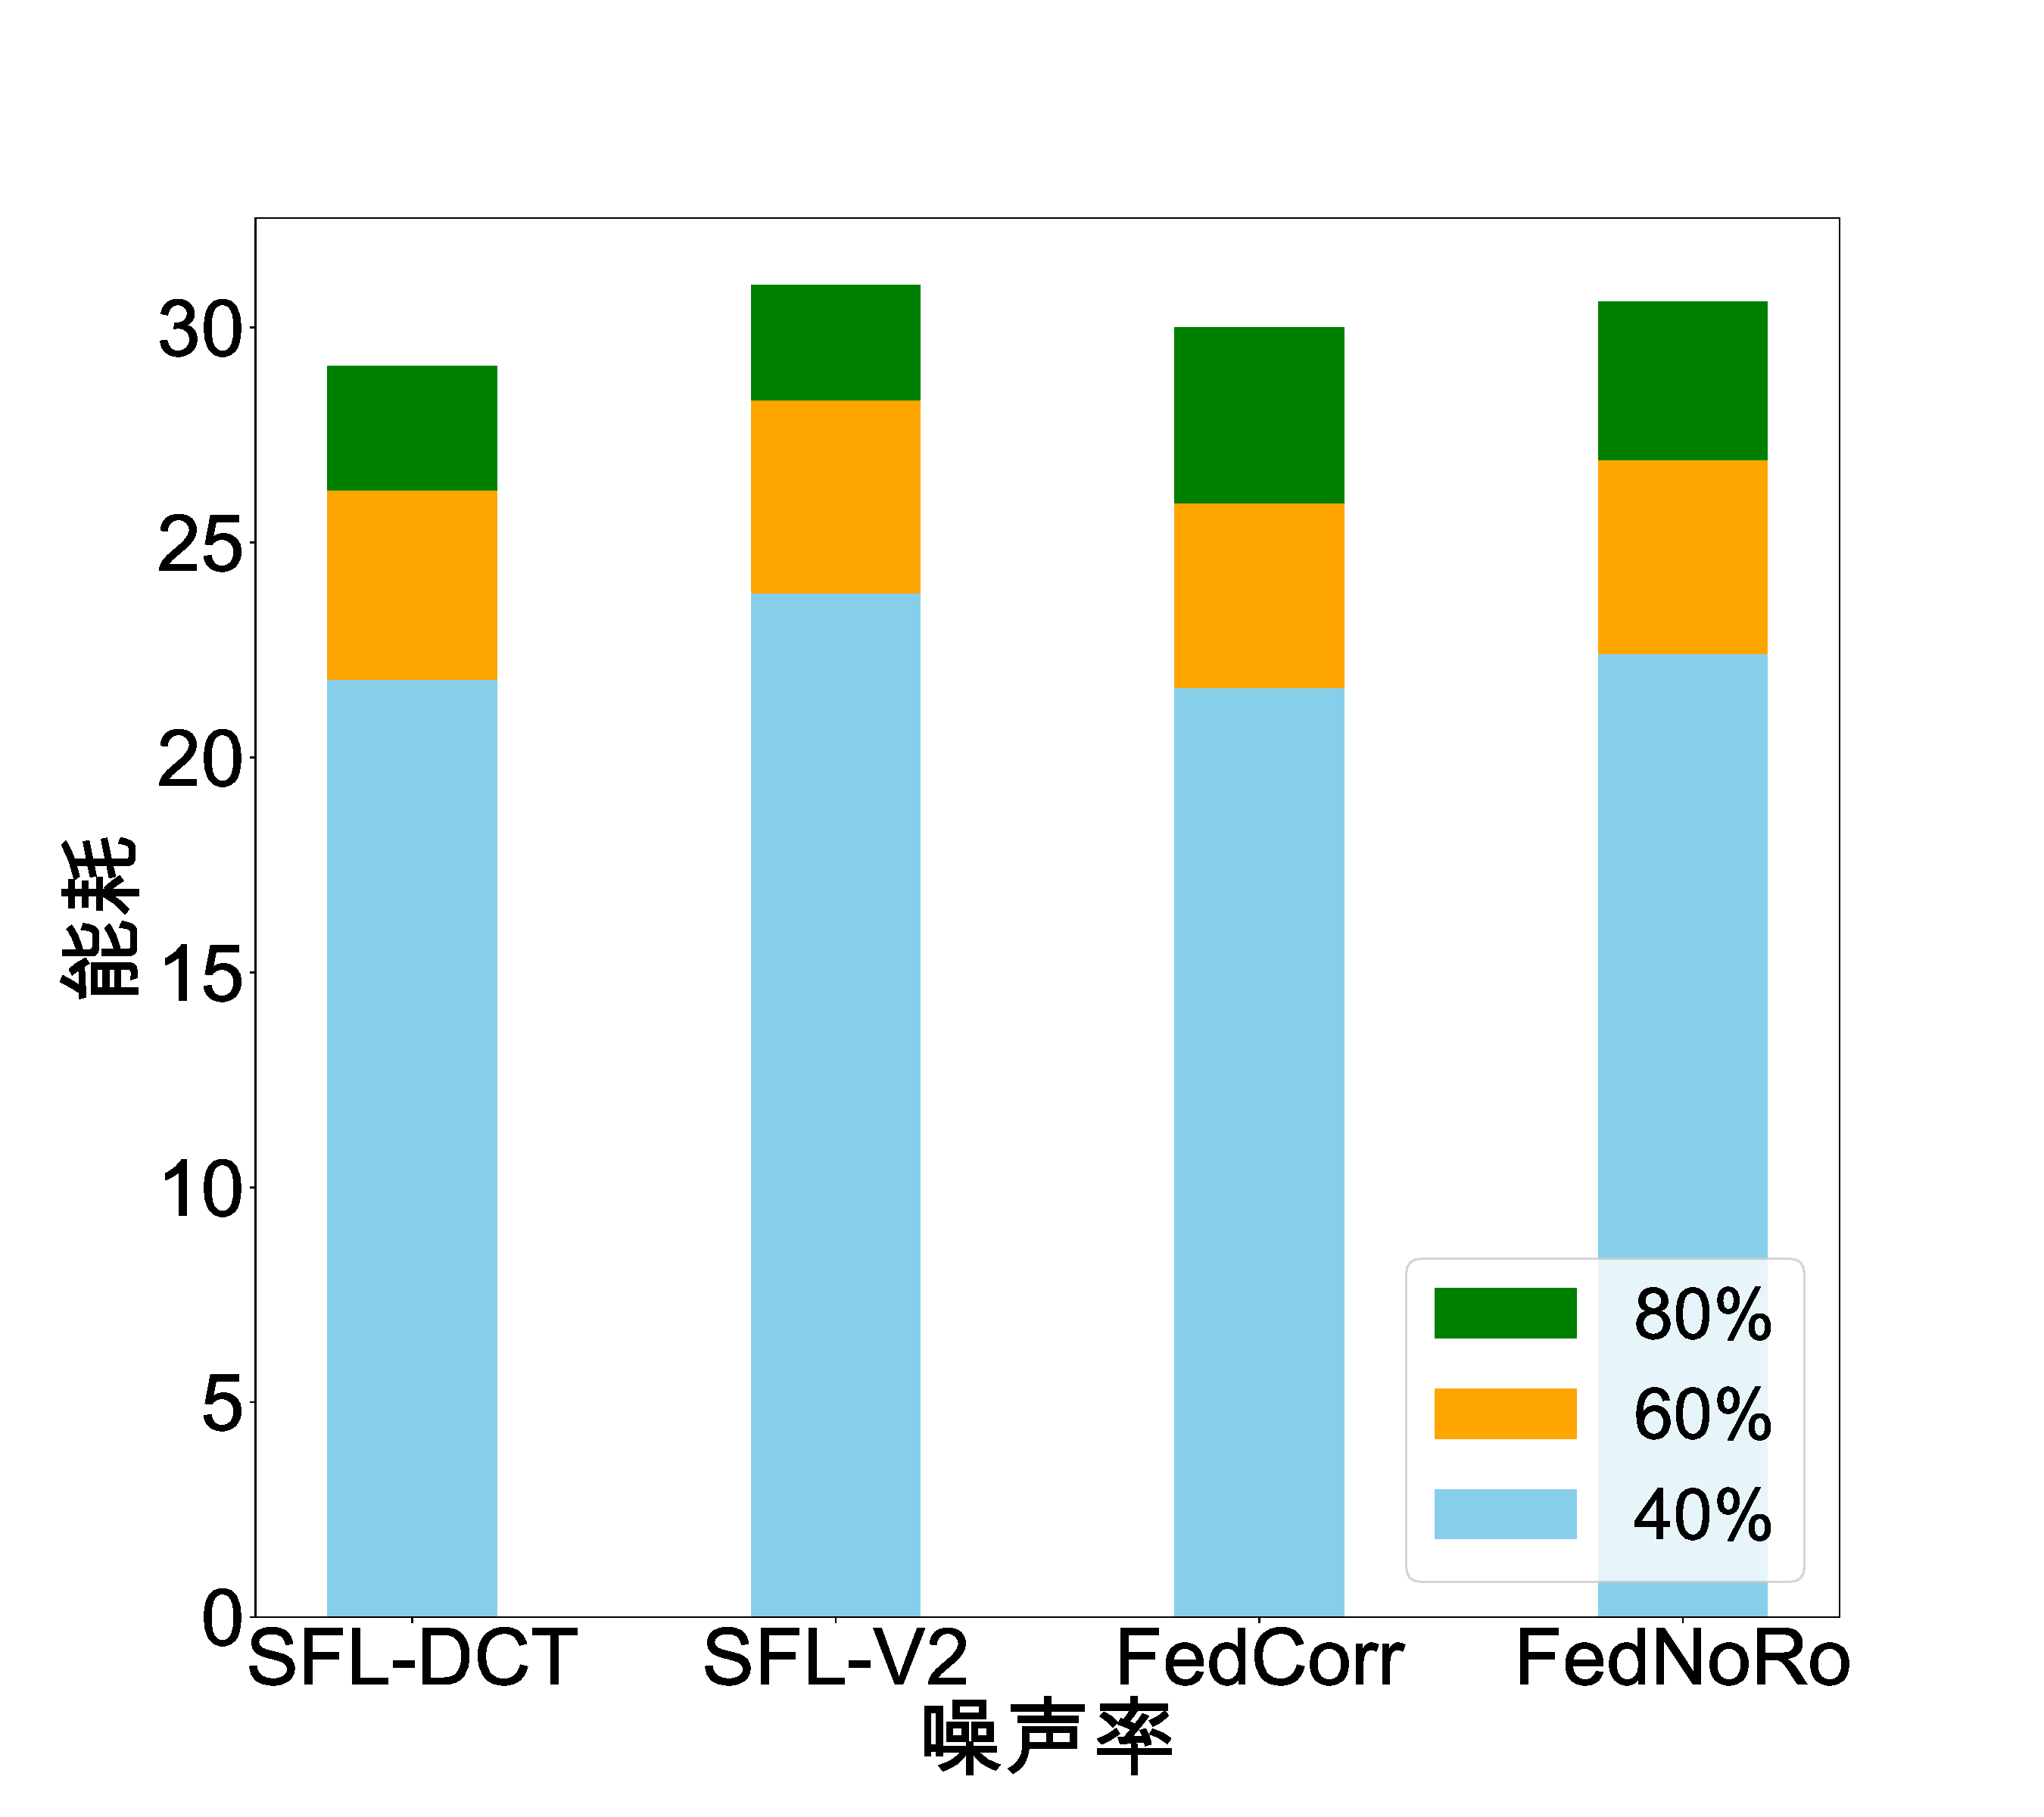
\includegraphics[width=\linewidth]{figures/power_iid.pdf}
\caption{Fashion-MNIST(IID)}
\label{fig:mnist_iid}
\end{subfigure}
\hfill
\begin{subfigure}{0.45\linewidth}
\centering
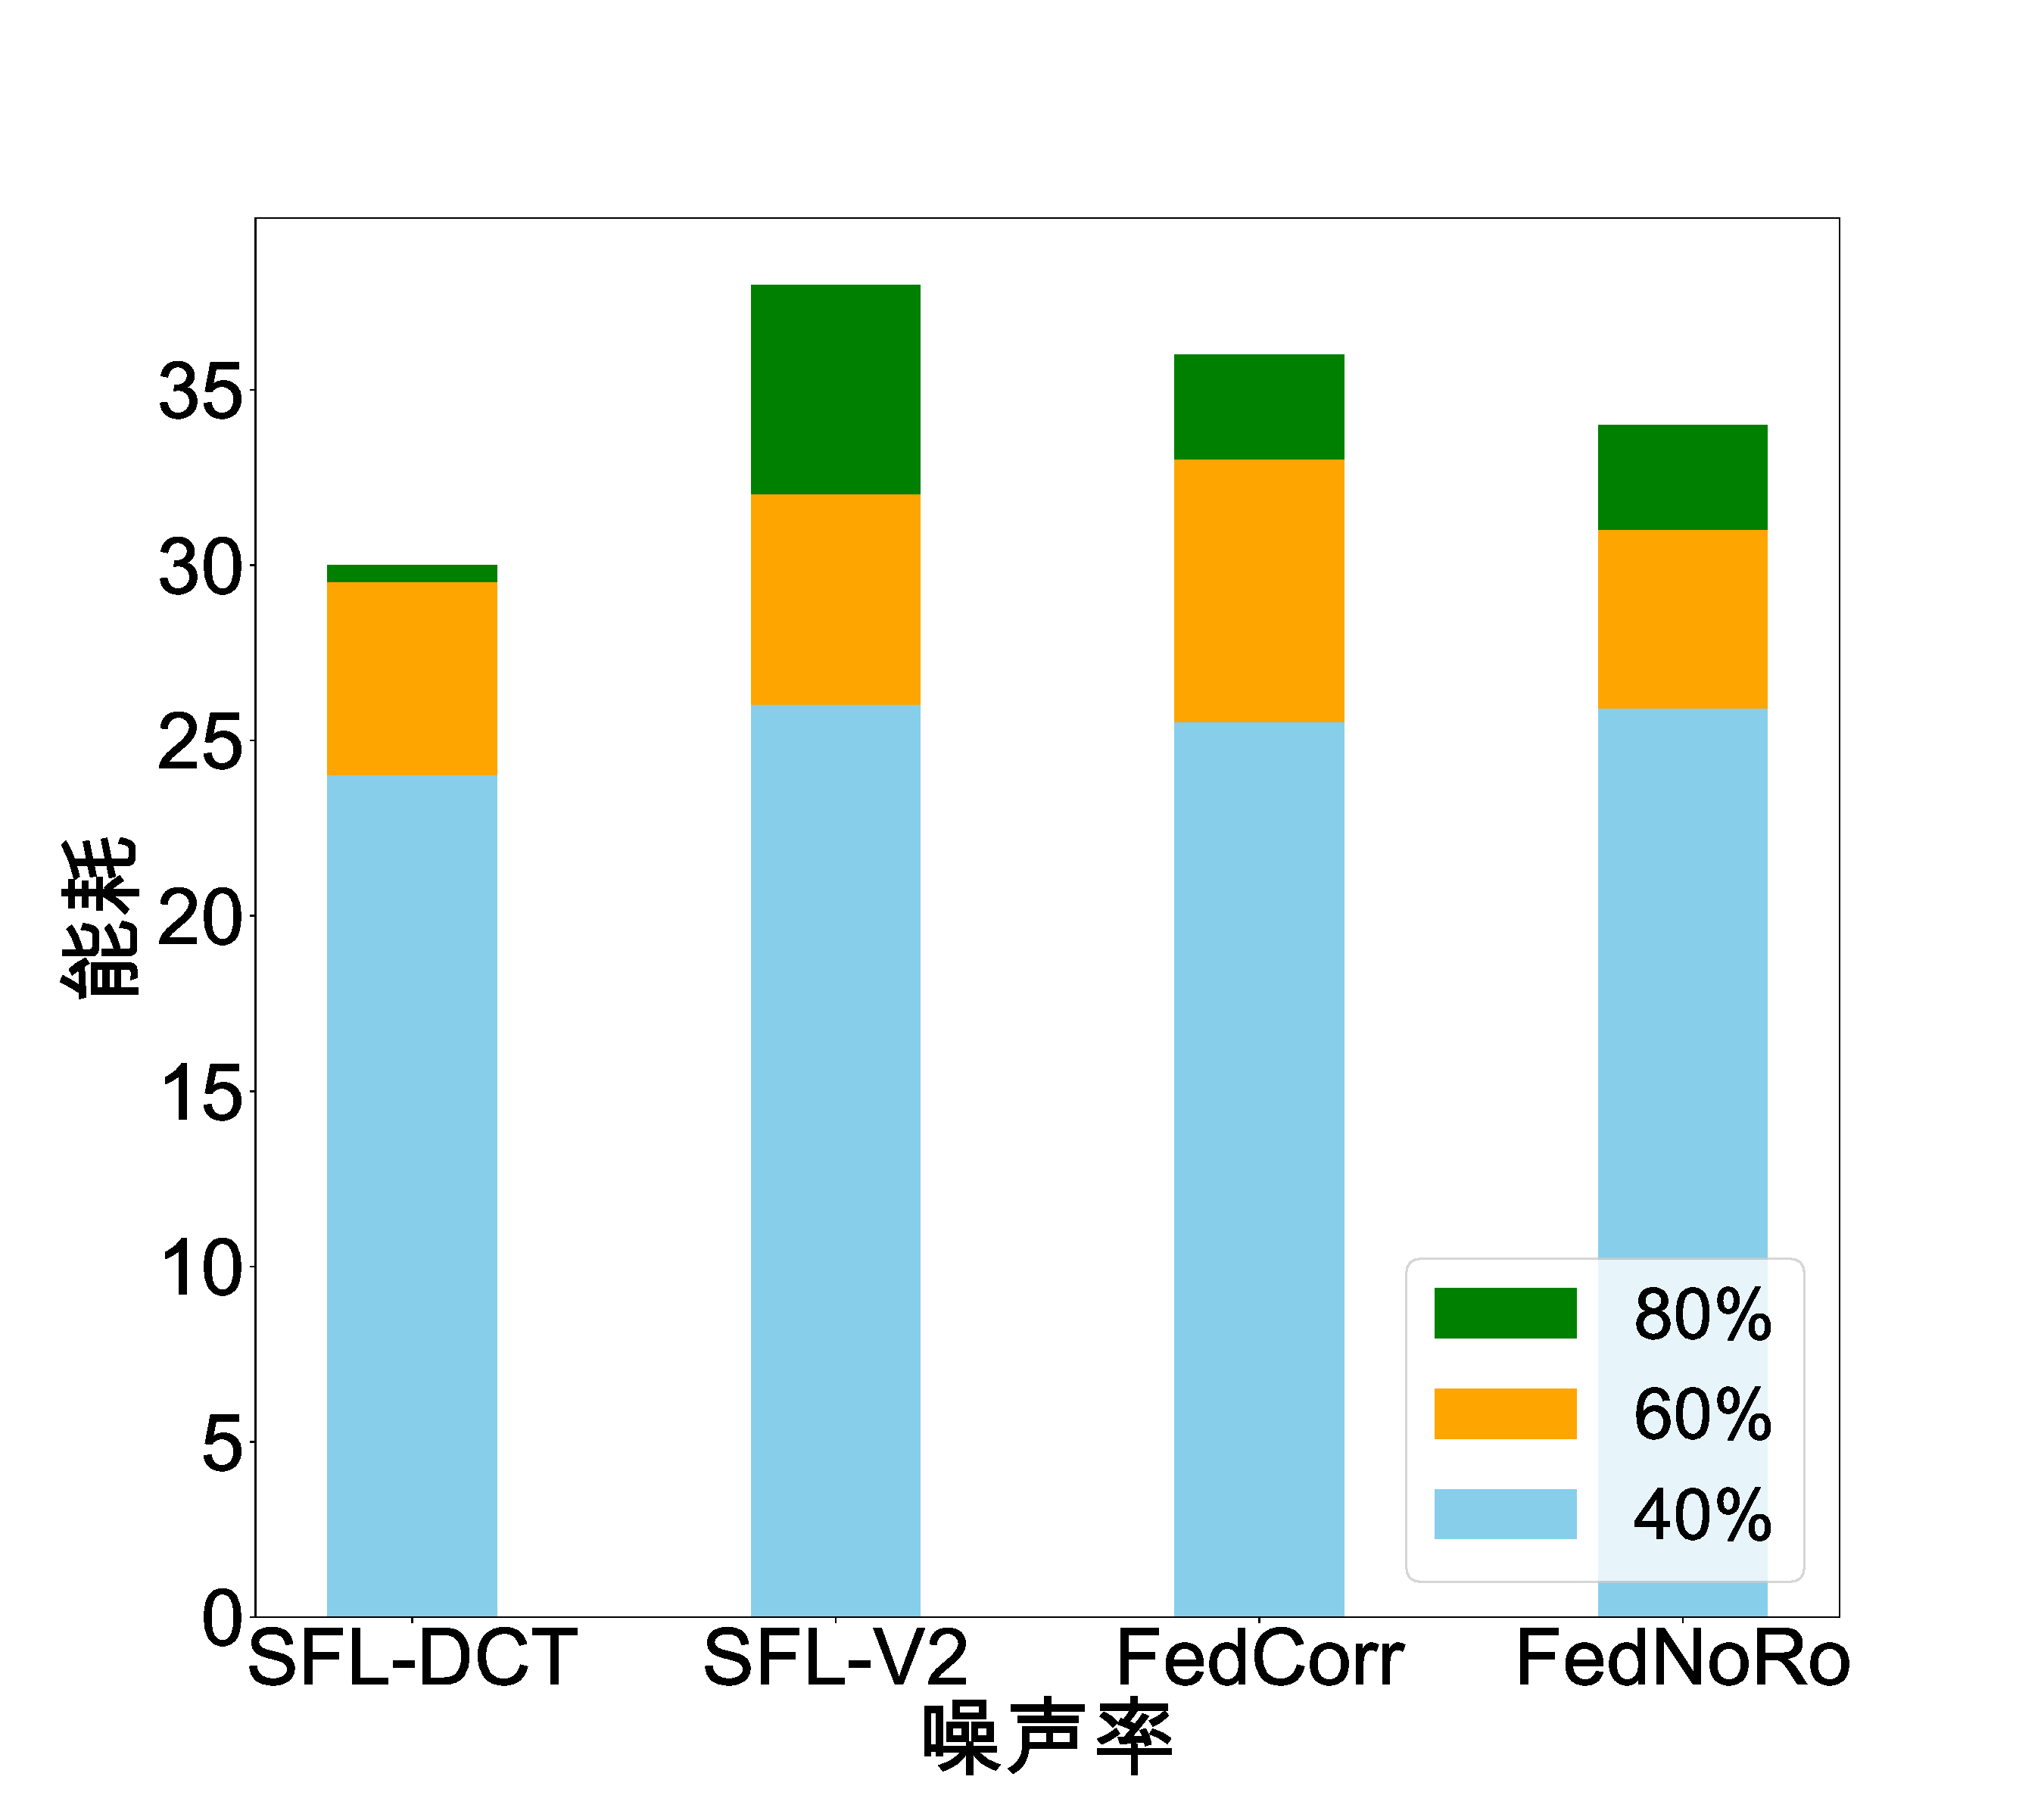
\includegraphics[width=\linewidth]{figures/power_noniid.pdf}
\caption{Fashion-MNIST(non-IID)}
\label{fig:mnist_noniid}
\end{subfigure}
\caption{不同算法的能量消耗对比。}
\label{fig:mnist_energy}
\end{figure}
\begin{table}[t]
\centering
\caption{分割-联邦学习与集中式学习中无反向传播训练方法的准确率比较}
\label{tab:bpfree n=10}
\begin{tabular}{c|cc}
\hline
\textbf{训练框架} & \textbf{模型} & \textbf{准确率 (\%)} \\ \hline
集中式学习 & ResNet-5 & 64.80 \\ \cline{2-3}
& VGG-8 & 74.30 \\ \hline
分割-联邦学习 & ResNet-5 & 62.22 \\ \cline{2-3}
& VGG-8 & 74.53 \\ \hline
\end{tabular}\label{tab:bpfree}
\end{table}
\subsection{SFL-DCT在测试平台上的能耗结果}



我们进一步在测试平台中评估了 SFL-DCT 和 SFL-V2 的实际收敛性和能耗（见第 \ref{sec:testbed} 节）。图 \ref{fig:testbed} 展示了我们的测试平台实验环境。在 SFL-DCT 中，我们将 $R_0$、$R_1$ 和 $R_2$ 设置得远小于 $R_3$，以使得对噪声标签的检测与纠正不会带来显著的计算开销。在每种设置下，我们测量了客户端直到 SFL-V2 收敛时所消耗的能量（单位为 kWh），以便进行公平比较，因为在收敛时 SFL-DCT 的准确率明显高于 SFL-V2。在这个系统中，一个 Raspberry Pi 代表一个客户端，而 PC 作为服务器，它们通过 WIFI 进行通信。我们选用 Fashion-MNIST 数据集，因为它适合计算能力受限的设备。如图 \ref{fig:mnist_energy} 所示，与 SFL-V2 相比，SFL-DCT 在客户端侧显著降低了能耗。在非独立同分布（non-IID）数据下，能耗降低最多可达 23.30\%。

\section{无反向传播训练的实验结果}
本实验在 CIFAR-10 数据集上，基于 ResNet-5 和 VGG-8 两种模型，评估了在分割式联邦学习框架中应用无反向传播训练方法的效果。实验中共有 10 个客户端参与。如表 \ref{tab:bpfree} 所示，采用无反向传播方法进行训练的分割式联邦学习，在测试准确率上接近于集中式训练下使用相同训练策略的结果。

